% SCTransform (v2) workflow for vignette 03-1, #fig-sc-transform.
% Panels: scripts/figures/fig_03_1_sctransform.R (ggplot2, seed 20261101).
% Build: latexmk -lualatex sctransform.tex; pdftocairo -svg sctransform.pdf
%        ../../fig_03_1_sctransform.svg
\documentclass[tikz,border=4pt]{standalone}
\usepackage{iftex}
\ifPDFTeX
  \PackageError{sctransform}{Use LuaLaTeX or XeLaTeX}{}
\fi
\usepackage{fontspec}
\usepackage{amsmath,amssymb,amsfonts,bm}
\usepackage{graphicx}
\usetikzlibrary{arrows.meta,positioning,fit,backgrounds,calc,shapes.geometric}
% palette and flowchart styles of vignettes/_quarto.yml
\definecolor{ink}{HTML}{1F2937}
\definecolor{latfill}{HTML}{DAE9FB}
\definecolor{latdraw}{HTML}{4477B5}
\definecolor{obsfill}{HTML}{C9CDD3}
\definecolor{obsdraw}{HTML}{747B86}
\tikzset{
  every node/.style={text=ink},
  edge/.style={-{Stealth[length=2.6mm]}, line width=0.8pt, draw=ink},
  box/.style={rectangle, rounded corners=3pt, draw=ink, fill=white, line width=0.8pt,
    align=center, inner sep=1.6mm, font=\small},
  keybox/.style={box, draw=latdraw, fill=latfill},
  dimbox/.style={box, draw=obsdraw, fill=obsfill!45},
  panel/.style={inner sep=0pt, anchor=north west},
  tag/.style={font=\bfseries\small, anchor=north west, inner sep=1pt}
}
\begin{document}
\begin{tikzpicture}
  % panels (3.1 x 2.6 in each)
  \node[panel] (A) at (0,0) {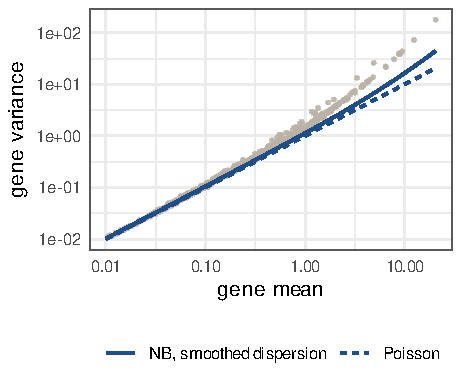
\includegraphics[width=7.4cm]{panel_a_mean_variance.pdf}};
  \node[panel] (B) at (9.2,0) {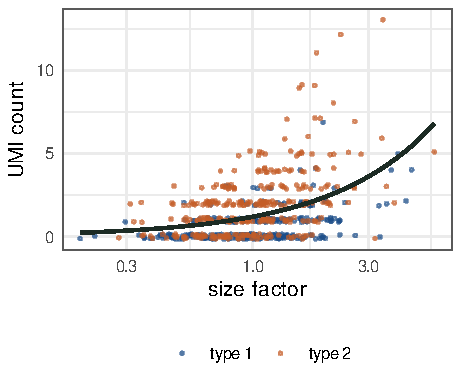
\includegraphics[width=7.4cm]{panel_b_depth.pdf}};
  \node[panel] (C) at (0,-8.4) {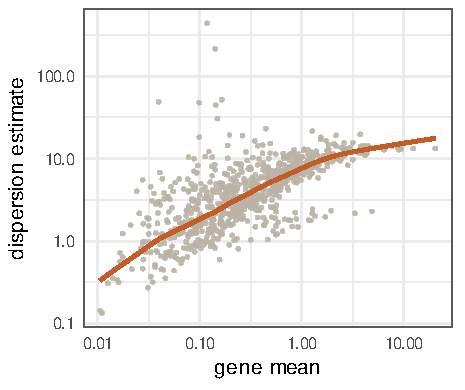
\includegraphics[width=7.4cm]{panel_c_regularisation.pdf}};
  \node[panel] (D) at (9.2,-8.4) {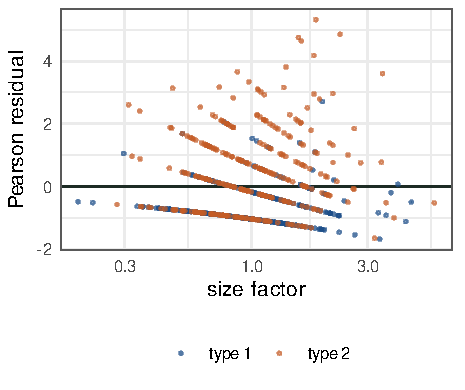
\includegraphics[width=7.4cm]{panel_d_residuals.pdf}};
  \node[tag] at (A.north west) {a};
  \node[tag] at (B.north west) {b};
  \node[tag] at (C.north west) {c};
  \node[tag] at (D.north west) {d};
  % notation above each panel
  \node[keybox, above=2mm of A, text width=7cm]
    (nA) {Negative-binomial variance\\
    $\operatorname{Var}(x_{gc})=m_{gc}+m_{gc}^{2}/\psi_g$};
  \node[keybox, above=2mm of B, text width=7cm]
    (nB) {Depth as an offset, no cell type ($M_0$)\\
    $\log m_{gc}=\beta_{0g}+\log s_c$};
  \node[keybox, above=2mm of C, text width=7cm]
    (nC) {Regularise across genes\\
    $\hat\psi_g\;\to\;\tilde\psi_g=\mathrm{smooth}\{\hat\psi_g\mid\log\bar x_g\}$};
  \node[keybox, above=2mm of D, text width=7cm]
    (nD) {Pearson residuals, clipped at $\pm\sqrt{C/30}$\\
    $r_{gc}=(x_{gc}-\hat m_{gc})\big/\sqrt{\hat m_{gc}+\hat m_{gc}^{2}/\tilde\psi_g}$};
  % flow
  \draw[edge] (A.south) -- node[right, font=\footnotesize, align=left]
    {one $\hat\psi_g$ per gene} (nC.north);
  \draw[edge] (B.south) -- node[right, font=\footnotesize, align=left]
    {fitted $\hat m_{gc}$} (nD.north);
  \draw[edge] (C.east) ++(0,0.6) -- node[above, font=\footnotesize] {$\tilde\psi_g$}
    ($(D.west)+(0,0.6)$);
\end{tikzpicture}
\end{document}
